\documentclass[preprint,12pt]{elsarticle}
\usepackage[T1]{fontenc}
\usepackage[utf8]{inputenc}
\usepackage{amsmath,amssymb,booktabs,tabularx}
\usepackage{graphicx}
\usepackage[hidelinks]{hyperref}
\usepackage{microtype}
\usepackage{listings}
\lstset{basicstyle=\ttfamily\small,breaklines=true,columns=fullflexible,frame=single}
\journal{Research software manuscript --- working draft}
\begin{document}
\begin{frontmatter}
\title{Random Clusters Generator: reproducible paired benchmarks for clustering with irrelevant features}
% Name from the repository metadata; author list and affiliations require confirmation.
\author{Jos\'e Mar\'ia Luna-Romera}
\begin{abstract}
Synthetic clustering experiments require more than a seed: comparisons must
preserve the intended signal while changing nuisance variables, distinguish
partition recovery from model selection, and expose Monte Carlo uncertainty.
Random Clusters Generator is an open-source Python package for balanced Gaussian
clusters with explicit signal and irrelevant coordinates. Its command-line
interface exports labelled data and provenance, while an optional research
workflow constructs paired experiments using separate random streams, matched
noise moments, immutable result directories and verifiable manifests. A case
study compares uniform and Gaussian irrelevant features under raw and
standardized preprocessing. An exploratory pilot motivates independent
validation and robustness scenarios varying sample size, dimensionality and
cluster number. The study examines known-cluster-count recovery separately from
selection by silhouette, Calinski--Harabasz and Davies--Bouldin indices. The
software provides an inspectable experimental scaffold for teaching, method
diagnostics and reproducibility studies; its balanced spherical model does not
represent the full diversity of clustering problems.
\end{abstract}
\begin{keyword}
Synthetic data \sep clustering \sep reproducibility \sep irrelevant features \sep simulation studies
\end{keyword}
\end{frontmatter}

\section{Motivation and significance}
In a clustering experiment, adding irrelevant variables should not silently
replace the informative observations or their labels. Conversely, obtaining a
high agreement score with a supplied cluster count does not establish that an
unsupervised procedure can discover that count. These requirements are simple
to state but easily obscured by scripts that regenerate data, change random
streams, or average correlated fits as independent observations.

Random Clusters Generator makes this small experimental workflow explicit. It
combines a documented generative model, command-line data export, a Python API,
paired perturbations and an auditable analysis pipeline. Its contribution is
the integration of these controls into an accessible research artifact, rather
than a new mixture model, clustering algorithm or internal validity index.
The intended users are researchers constructing diagnostic examples and
educators demonstrating the distinction between data geometry and evaluation.

Existing tools have broader modelling capabilities. The scikit-learn
\texttt{make\_blobs} function generates isotropic Gaussian clusters and accepts
explicit centers \cite{makeblobs,sklearn}; our conditional signal distribution
can therefore be reproduced with this standard building block. MixSim controls
mixture overlap and supports noise variables and outliers \cite{mixsim}.
HAWKS evolves benchmark datasets to satisfy properties or challenge algorithms
\cite{hawks}. We do not claim broader coverage or better generation quality
than these tools. Here, fixed signal realizations, nested nuisance columns,
paired distributional changes, raw fit records and uncertainty summaries are
packaged together for a deliberately restricted model.

The closest substantive antecedent is McCrory and Thomas \cite{mccrory2024},
who investigate irrelevant uniform/Gaussian variables, scaling and clustering
metrics on Dimsets. Thus, noise sensitivity itself is not a novelty claim.
Our case study emphasizes equal population noise moments and the distinction
between known-count partition recovery and label-free count selection.
The protocol follows the aims, data-generating mechanisms, estimands, methods
and performance-measures structure of simulation-study guidance
\cite{morris2019}. Claims are conditional on the benchmark design, consistent
with clustering benchmarking recommendations \cite{vanmechelen2023}.

\section{Software description}
\subsection{Architecture and interfaces}
The package separates three concerns. The core validates an immutable
configuration and generates a table with centers and resolved seed. The I/O
layer exports CSV and JSON metadata, including parameters, versions and a file
checksum. The command-line layer exposes \texttt{generate}, \texttt{batch} and
\texttt{add-noise}. A separate optional research package implements paired
families, model fitting and reports. Basic generation depends only on NumPy
and pandas; the research extra adds scikit-learn, SciPy, Matplotlib and
threadpoolctl. The package requires Python 3.10 or later and uses an MIT license.

Tests cover parameter rejection, deterministic replay, row and label
preservation, output protection and paired streams. A reduced end-to-end
research test exercises generation, fitting, selection and report integrity.
Continuous integration checks three operating systems and Python versions
3.10, 3.12 and 3.13, minimum core dependencies, and a research environment.
An integrity checker verifies archived artifact hashes independently of the
optional modelling libraries. Tests establish implementation properties;
they do not establish scientific validity for every application.

\subsection{Data-generating model}
Let $k$ denote the number of groups, $m$ observations per group, $p$ signal
coordinates and $q$ added irrelevant coordinates, so $n=km$. Distinct centers
$\mu_c$ are sampled without replacement from $\{0.25,0.75\}^{p}$, requiring
$k\leq 2^p$. Conditional on group $c$,
\begin{equation}
 S_i=\mu_c+\sigma Z_i,\qquad Z_i\sim N_p(0,I_p),\qquad
 X_i=(S_i,N_i).
\end{equation}
The basic generator draws each coordinate of $N_i$ independently from
$U[0,1)$. Labels are available for evaluation and must be excluded from input
features. Columns are named \texttt{s0}, \texttt{s1}, etc., for signal,
\texttt{d0}, \texttt{d1}, etc., for noise, and \texttt{cluster} for the label.
Coordinates named signal need not all distinguish the selected centers; the
research diagnostics record which actually vary. Gaussian observations are
unbounded and are not clipped to the unit cube.

The research design also uses $N(0.5,1/12)$ noise, matching the uniform mean
and variance. For a uniform draw $U$, its paired Gaussian counterpart is
$0.5+\Phi^{-1}(U)/\sqrt{12}$; inverse-transform endpoints are numerically
clipped. Within a replicate, signal residuals, centers, labels and permutation
remain fixed as $q$ changes; smaller noise matrices are exact column prefixes
of larger ones. Separate PCG64 streams are keyed by master seed, replicate,
geometry, component and column using NumPy SeedSequence \cite{numpyparallel}.
Preprocessing variants share data and algorithm seeds. Equal moments do not
make the two noise distributions geometrically equivalent.

The public generator and research family have distinct random-stream designs.
An identical integer seed across these interfaces does not promise identical
tables. Exact replay requires the recorded design, configuration and numerical
environment, rather than an assumption of cross-version bitwise stability.

\section{Illustrative use and experimental design}
\subsection{From configuration to inspectable data}
After cloning the repository and installing with \texttt{python -m pip install .},
a first dataset is generated as follows:
\begin{lstlisting}
random-clusters generate --clusters 4 --samples 100
  --features 2 --noise 2 --std 0.05 --seed 42
  --output data/demo.csv
\end{lstlisting}
The displayed command should be entered on one line. It produces 400 rows,
four feature columns and one label column, together with \texttt{demo.json}.
The \texttt{samples} argument counts observations per group. Existing outputs
are protected unless overwrite is explicitly requested. Batch input is a CSV
table of named configurations; the README gives input and output examples in
English and Spanish. The research workflow runs from a JSON configuration:
\begin{lstlisting}
python -m pip install ".[research]"
python -m random_clusters.research.run
  --config research/validation-primary.json
  --protocol research/VALIDATION_PROTOCOL.md
  --output data/validation-primary
python -m random_clusters.research.report data/validation-primary
\end{lstlisting}
Each invocation is entered on one line. Outputs include dataset fingerprints,
all fits, count selections, a predefined CSV gallery and regenerable figures.
This separates generating evidence from rendering summaries.

\subsection{Case study}
An exploratory pilot used 20 independent families, $k=4$, $p=2$, $m=100$,
$\sigma\in\{0.05,0.15,0.30\}$ and $q\in\{0,2,8,32\}$. Each positive $q$
had both noise laws; $q=0$ was generated once. It produced 420 datasets,
6,720 fits and 2,520 index-based selections. The two executions used to audit
replay are not additional independent replicates.

The pilot motivated a separately seeded validation with 200 families,
$k=4$, $p=2$, $m=100$, $\sigma=0.05$ and $q\in\{0,2\}$. Its primary
estimand is the paired normal-minus-uniform difference in probability that
silhouette selects $k=4$ after standardization at $q=2$. The maximum Monte
Carlo standard error for each marginal success proportion is 0.0354; precision
of the paired contrast is estimated from its own replicate differences.
Three robustness scenarios use 50 families each and the full pilot
$\sigma,q$ grid: $(k,p,m)=(4,2,50),(4,4,100),(8,3,50)$. They change sample
size, partial-cube geometry and full-cube cluster count, respectively. The last
changes $k$ and $p$ jointly; it cannot isolate a cluster-count effect.

For each raw or feature-standardized dataset, Lloyd K-means uses k-means++,
10 initializations, tolerance $10^{-4}$ and at most 300 iterations. Candidate
counts are 2--8, extended to 2--12 for the eight-group scenario. Silhouette and
Calinski--Harabasz are maximized; Davies--Bouldin is minimized. Exact ties choose
the smaller count. Labels never enter these selection rules. K-means with the
generating count and Ward agglomeration at that count provide separate
known-count evaluations. All metrics use Euclidean geometry; silhouette is
computed on every observation, without subsampling.

Adjusted Rand index (ARI) is the main external endpoint; normalized mutual
information is also archived. The signed selection difference is
$\mathrm{ARI}(\widehat{k})-\mathrm{ARI}(k)$, which need not be nonpositive.
For replicate contrasts $D_r$, we report $\overline D$,
$\mathrm{MCSE}=s_D/\sqrt R$ and pointwise 95\% Student-$t$ intervals.
Success proportions use Wilson intervals. Replicate families, rather than
rows, candidate fits or preprocessing conditions, are the independent units.
No multiplicity-adjusted inference or universal algorithm ranking is intended.
Protocols and seeds were committed before their respective executions;
the validation protocol was informed by the pilot and was not externally
preregistered. All failures and warnings are retained.

\section{Results and interpretation}
The exploratory pilot showed perfect known-count recovery at $\sigma=0.05$
without added noise. At $q=2$, mean raw K-means ARI was 0.237 for uniform noise
and 0.545 for Gaussian noise; the paired difference was 0.308 (95\% interval
0.181--0.435). After standardization, the corresponding means were 0.970 and
0.999, yet silhouette selected the generating count in 0/20 uniform and 19/20
Gaussian cases. These exploratory observations motivated the independently
seeded validation specified above. Its results and robustness checks will be
inserted from the archived run records after completion and verification.

\begin{figure}[htbp]
\centering
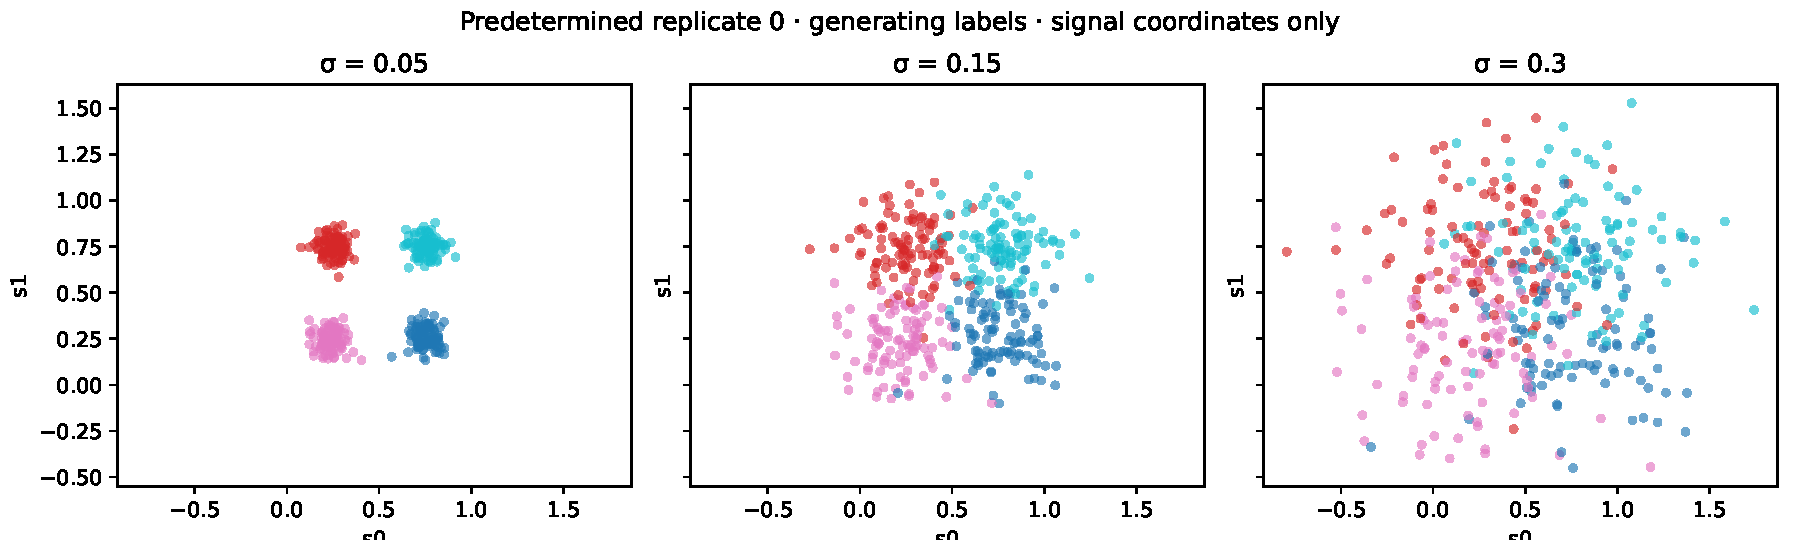
\includegraphics[width=\textwidth]{gallery.pdf}
\caption{Predefined pilot gallery, replicate zero. Each panel shows the first
two signal coordinates, colored by generating label. Adding irrelevant columns
preserves these points; their unchanged appearance is the intended paired
control, not a projection of a changed clustering solution. The exported CSVs
contain the additional coordinates.}
\label{fig:gallery}
\end{figure}


\section{Impact, limitations and reuse}
The practical result is a reusable route from a small configuration to
datasets, paired comparisons, uncertainty estimates and inspectable evidence.
Researchers can substitute a clustering method while keeping the data families,
or extend a noise grid without altering already defined columns. The gallery
supports teaching, while raw candidate fits permit alternative summaries
without rerunning the algorithms. These are supported use cases, not evidence
of external adoption; no independent user-impact study has been performed.

The generator intentionally excludes unequal group sizes, anisotropy,
correlated nuisance variables, missing values, outliers and nonconvex shapes.
Its geometry favors some clustering objectives. Increasing $\sigma$ changes
both overlap and marginal signal variance, so raw-scale comparisons do not
isolate overlap alone. Standardization gives each variable unit empirical
variance but cannot make irrelevant coordinates informative. A lower internal
score is not, by itself, proof that an index is defective: each index optimizes
a geometric criterion rather than recovery of the generating labels.

Finite candidate ranges may create boundary preferences, and ten K-means
starts do not guarantee the global optimum. The experiments do not benchmark
speed or memory against other generators. Exact silhouette requires a dense
pairwise distance matrix, with quadratic memory in the number of observations;
large-data applications need a separately validated approximation. Reproducible
synthetic diagnostics complement, rather than replace, domain-specific data
and broader benchmark families.

\section{Conclusions}
Random Clusters Generator packages a restricted, transparent mixture model
with practical provenance and paired experimental controls. Separating
known-count recovery from count selection makes its case study useful for
diagnosing what a clustering evaluation actually measures. The artifact is
designed to be inspected, replayed and extended, with claims limited to the
documented data-generating mechanisms.

\section*{Code and data availability}
Source code, protocols, dependency versions, raw experimental records and
checksums are available at
\url{https://github.com/josemarialuna/RandomClustersGenerator}.
Individual run manifests identify their exact source revisions. Representative
datasets are included; all others are regenerated from archived configurations.
The software is licensed under MIT. No human-subject data are used.

\section*{Declaration of generative AI assistance}
OpenAI's coding assistant was used to assist software implementation,
experimental scripting, literature discovery, manuscript drafting and formatting.
Numerical claims are derived from archived executable experiments. Human
verification and approval of the manuscript, references, authorship and
submission declarations are required before submission.

\bibliographystyle{elsarticle-num}
\bibliography{references}
\end{document}
